\chapter{Einführung}
\label{chap:einfuehrung}

\section{Zusammenfassung}

\subsection{Überblick}
\begin{figure}[htdp]
	\center
	\begin{tikzpicture}[very thick,
		node distance=2.5cm,on grid,>=stealth',
		block/.style={rectangle,draw,rounded corners=1mm,minimum height=1cm,minimum width=2cm}]

\node [block] (top)						{Mathematik};
\node [block] (down3) [below=of top]	{Analysis} edge [-] (top);
\node [block] (down2) [left=of down3]	{Algebra} edge [-] (top);
\node [block] (down1) [left=of down2]	{\begin{tabular}{c}Logik und\\ Mengenlehre\end{tabular}} edge [-] (top);
\node [block] (down4) [right=of down3]	{Stochastik} edge [-] (top);
\node [block] (down5) [right=of down4]	{Numerik} edge [-] (top);
\end{tikzpicture}

	\caption{Teilgebiete der Mathematik}
\end{figure} 

\textbf{Definitionsversuch:} Entwicklung und mathematisches Verständnis von numerischen Algorithmen, als von Rechenmethoden zur zahlenmäßigen Lösung mathematischer Probleme.

\textbf{Zusammenspiel mit Informatik:}
\begin{figure}[htdp]
	\begin{tikzpicture}[very thick,node distance=1.5cm,on grid,>=stealth']
\node (top)	{Numerische Mathematik};
\node (mid) [below=of top] {\begin{tabular}{l}Scientific Computing\\ Wissenschaftliches Rechnen\end{tabular}} edge [<-] (top);
\node (down) [below=of mid]	{Informatik} edge [<-] (mid);
\node [node distance=7cm, right=of mid] {\begin{tabular}{c}Logik und\\ Mengenlehre\end{tabular}} edge [<-] node [midway,above] {Computer} (mid);
\end{tikzpicture} 

	\caption{Zusammenspiel Mathematik und Information in der Numerik}
\end{figure}

\subsection{Vorgehen}
\begin{figure}[htdp]
	\center
	\begin{tikzpicture}[very thick,node distance=1.5cm,on grid,>=stealth']
	\node (top)	{Anwendungsproblem};
	\node (down1) [below=of top] {Primäres mathematisches Problem} edge [<-] node [right] {Mathematisierung} (top);
	\node (down2) [below=of down1] {Sekundäre mathematische Probleme} edge [<-] node [right] {Mathematische Umformungen} (down1);
	\node (down3) [below=of down2] {Algorithmus/Computerprogramm} edge [<-] node [right] {Programmierung} (down2);
	\node (down4) [below=of down3] {"'Lösung"'} edge [<-] node [right] {Rechnung} (down3);
	\node [below=of down4] {Lösung} edge [<-] node [right] {Beurteilung, "'Entmathematisierung"'} (down4);
\end{tikzpicture} 

	\caption{Vorgehen zur Lösung eines mathematischen Problems}
\end{figure}

\subsection{Aspekte für die Lösung einer mathematischen Aufgabenstellung}
\begin{itemize}
	\item Kondition eines Problems (Empfindlichkeit für Störungen)
	\item Numerische Lösungsverfahren
	\item Stabilität des Lösungsverfahrens (Empfindlichkeit für Störungen)
	\item Effizienz des Lösungsverfahrens
	\item Genauigkeit der Lösung
\end{itemize}

\section{Wiederholung}

\subsection{Lineares Gleichungssystem}

\begin{align*}
	a_{11}\,x_1 + \ldots + a_{1n}\,x_n &= b_1\\
	a_{21}\,x_1 + \ldots + a_{2n}\,x_n &= b_2\\
	&\vdots\\
	a_{m1}\,x_1 + \ldots + a_{mn}\,x_n &= b_m\\
	\ma{A} \cdot \vec{x} &= \vec{b}\\
	\ma{A} &\in \mathbb{R}^{m\times n},\ \vec{x} \in \mathbb{R}^n,\ \vec{b} \in \mathbb{R}^m
\end{align*}

\subsection{Matrizen}
\subsubsection{Elementare Matrix-Operationen}


\textbf{Addition:}
\begin{align*}
	\ma{A}_{<m\times n>} + \ma{B}_{<m\times n>} &= \ma{C}_{<m\times n>}\\
	c_{\mu\nu} &= a_{\mu\nu} + b_{\mu\nu}
\end{align*}

\textbf{Multiplikation mit Skalar:}
\begin{align*}
	k \cdot \ma{A} = \ma{A} \cdot k = B\\
	b_{\mu\nu} = k \cdot a_{\mu\nu}
\end{align*}

\textbf{Matrix-Multiplikation:}
\begin{align*}
	\ma{A}_{<m\times n>} \cdot \ma{B}_{<n\times l>} &= \ma{C}_{<m\times l>}\\
	c_{\mu\nu} &= \sum_{\nu=1}^{n} a_{\mu\nu} \cdot b_{\mu\lambda};\quad \mu=1\ldots m,\ \lambda=1\ldots l
\end{align*}

\textbf{Multiplikation Matrix-Vektor:}
\begin{align*}
	\text{Spezialfall der Matrix-Multiplikation: } <n\times 1> \text{ bzw. } <1\times n>
\end{align*}

\textbf{Auffassen als Linearkombination der Spalten der Matrix:}
\begin{align*}
	\ma{A} \cdot \vec{x} &= \vec{b}\\
	\begin{bmatrix}\vec{a}_1 & \vec{a}_2 & \ldots & \vec{a}_n\end{bmatrix} \cdot \vec{x} &= \vec{b}\\
	\vec{a}_1\,\vec{x} + \ldots + \vec{a}_n\,\vec{x}_n &= \vec{b}
\end{align*}

\textbf{Vektoren:}
\begin{align*}
	\text{Spaltenvektor:} \quad & \vec{a}_{<n\times 1>}: \vec{a}\\
	\text{Zeilenvektor:} \quad & \vec{b}_{<1\times m>}^T: \vec{b}^T
\end{align*}

\subsubsection{Vektormultiplikation}
\begin{align*}
	\vec{b}^T\cdot \vec{a} &= c \quad \text{(Skalarprodukt $m=n$!)}\\
	\vec{a} \cdot \vec{b}^T &= \ma{C} \quad \text{(Vektorprodukt, dyadisches Produkt)}
\end{align*}

\textbf{Matrix als Kombination von Zeilen- und Spaltenvektoren:}
\begin{align*}
	\ma{A}_{<m\times n>} &= \begin{bmatrix} \vec{a}_1^T \\ \vec{a}_2^T \\ \vdots \\ \vec{a}_m^T \end{bmatrix}\\
	\ma{B}_{<n\times l>} &= \begin{bmatrix} \vec{b}_1 & \vec{b}_2 & \ldots & \vec{b}_l \end{bmatrix}\\
	\ma{A} \cdot \ma{B} &= \ma{C}\\
	\vec{c}_{\mu\lambda} &= \vec{a}_\mu^T \cdot \vec{b}_\lambda
\end{align*}

\textbf{Rechenregeln:}
\begin{align*}
	\left(\ma{A}\cdot \ma{B}\right)\cdot \ma{C} &= \ma{A} \cdot \left(\ma{B} \cdot \ma{C}\right) \quad \text{Assoziativität}\\
	\ma{A} \cdot \left(\ma{B} + \ma{C}\right) &= \ma{A}\,\ma{B} + \ma{A}\,\ma{B} \quad \text{Distributivität}\\
	\ma{A} \cdot \ma{B} &\neq \ma{B} \cdot \ma{A} \quad \text{Kumutativität gilt im Allgemeinen nicht}
\end{align*}

\textbf{Diagonalmatrix:}
\begin{align*}
	\ma{D} &= \text{diag}\begin{bmatrix}d_1 & d_2 & \ldots & d_n\end{bmatrix} = \begin{bmatrix}d_1 & \ldots & 0 \\ 0 & \ldots & d_n\end{bmatrix}\\
	\ma{D}_1 \cdot \ma{D}_2 &= \ma{D}_2 \cdot \ma{D}_1
\end{align*}

\textbf{Einheitsmatrix:}
\begin{align*}
	\ma{I} = \ma{E} = \ma{1} = \text{diag}\begin{bmatrix}1 & \ldots & 1\end{bmatrix}\\
	\ma{A} \cdot \ma{I} = \ma{I} \cdot \ma{A}\\
	\ma{I}^n = \ma{I}\\
	\ma{I}^{-1} = \ma{I}
\end{align*}

\textbf{Transponierte Matrix:}
\begin{align*}
	\ma{A}_{<m\times n>}^T &= \ma{B}_{<n\times m>},\ b_{\nu\mu} = a_{\mu\nu}\\
	\left(\ma{A} \cdot \ma{B}\right)^T &= \ma{B}^T \cdot \ma{A}^T\\
	\ma{A} &= \ma{A}^T \quad \Rightarrow \text{ symmetrische Matrix}
\end{align*}

\textbf{Inverse Matrix:}
\begin{align*}
	\ma{A} &\in \mathbb{R}^{n\times n}\\
	\ma{A}^{-1} \cdot \ma{A} &= \ma{A} \cdot \ma{A}^{-1} = \ma{I}\\
	\text{$\ma{A}^{-1}$ existiert nur für nicht singuläre $\ma{A}$}&\text{ und ist eindeutig.}\\
	\ma{A} = \text{diag}\begin{bmatrix}d_1 & \ldots & d_n\end{bmatrix} & \Rightarrow \ma{A}^{-1} = \text{diag}\begin{bmatrix}\frac{1}{d_1} & \ldots & \frac{1}{d_n}\end{bmatrix}\\
	\left(\ma{A} \cdot \ma{B}\right) &= \ma{B}^{-1} \cdot \ma{A}^{-1}
\end{align*}

\section{Schaltungsanalyse}
\begin{figure}[htdp]
	\center
	\begin{circuitikz}
	\draw
		(0,4)
		to [R=$Y_1$, i=\textcolor{green!70!blue}{$i_1$},-o] (4,4) node[above] {1}
		to [R=$Y_3$, i=\textcolor{green!70!blue}{$i_3$},v>=\textcolor{blue}{$u_3$},-o] (8,4) node[above] {3}
		to [R=$Y_5$, i<^=\textcolor{green!70!blue}{$i_5$},v=\textcolor{blue}{$u_5$},o-o] (12,4) node[above] {2} 
		to [short,i<=\textcolor{green!70!blue}{$i_2$}] (12,3)
		to [R=$Y_2$,v=\textcolor{blue}{$u_2$},*-*] (12,1)
		to (13.5,1)
		to [I,i_=$I_{02}$] (13.5,3) to (12,3)
		(12,1) to (12,0) to (8,0) node[ground] {}
		to [R=$Y_4$, i=\textcolor{green!70!blue}{$i_4$},v>=\textcolor{blue}{$u_4$},o-] (8,4) 
		(8,0) +(0.2,0) node[above] {0} to (0,0)
		to [V=$U_{01}$] (0,4)
		(4,4) 
		to [open,v=\textcolor{blue}{$u_1$}] (0,0);
	
	\draw[color=red](8,0)
		to [open,v^>=\textcolor{red}{$u_{n1}$}] (4,4)
		(9,0)
		to [open,v>=\textcolor{red}{$u_{n3}$}] (9,4)
		(11,0)
		to [open,v^>=\textcolor{red}{$u_{n2}$}] (11,4);
\end{circuitikz} 

	\caption{Beispielschaltung}
\end{figure}
\begin{tabular}{llll}
	\textcolor{green!70!blue}{$\vec{i}_{<k>}$} & \textcolor{green!70!blue}{Kantenstromvektor} & \textcolor{blue}{$\vec{u}_{<k>}$} & \textcolor{blue}{Kantenspannungsvektor}\\
	$\vec{i}_{0<k>}$ & Kantenquellenstromvektor & $\vec{u}_{0<k>}$ & Kantenquellenspannungsvektor\\
	$\vec{i}_{n<k>}$ & Knotenquellenstromvektor & \textcolor{red}{$\vec{u}_{n<k>}$} & \textcolor{red}{Knotenquellenspannungsvektor}\\
	\\
	$\ma{A}_{<n\times k>}$ & Kontenmatrix, Knoteninzidenzmatrix & &\\
	$\ma{Y}_{<k\times k>}$ & Kantenadmittanzmatrix & &\\
	$\ma{Y}_{n<n\times n>}$ & Kontenadmittanzmatrix & &\\
\end{tabular}

\subsection{Gerichteter Graph der Schaltung}

\subsection{Inzidenz Matrix}
\begin{align*}
	\ma{A}_{<m\times n>} = \begin{bmatrix}
	1 & & & -1\\
	 & 1 & & -1\\
	-1 & & 1 & \\
	 & & 1 & -1\\
	 & -1 & 1 & 
	\end{bmatrix}
\end{align*}
Summen der Spaltenvektoren $= \vec{0}$.\\
$\Rightarrow \ma{A}$ hat linear abhängige Spalten.

Rang der Matrix $\ma{A}$: $r = \rang{\ma{A}} = 3 = n-1$.\\
Dimension des Nullraums: Zahl der Spalten $-\ r = 1$ .\\
Vektor im Nullraum von $\ma{A}$:
\begin{align*}
	\ma{A}\cdot\vec{u}=\vec{0}\Rightarrow\vec{u}\in ;\quad\vec{u}=\begin{bmatrix}1\\1\\1\\1\end{bmatrix}
\end{align*}

\subsection{Laplace Matrix}
\begin{align*}
	\ma{A}^T\cdot\ma{A} = \begin{bmatrix}
	1 & 0 & -1 & 0 & 0\\ 
	0 & 1 & 0 & 0 & -1 \\ 
	0 & 0 & 1 & 1 & 1 \\ 
	-1 & -1 & 0 & -1 & 0
	\end{bmatrix}\cdot\begin{bmatrix}
	1 & 0 & 0 & -1 \\ 
	0 & 1 & 0 & -1 \\ 
	-1 & 0 & 1 & 0 \\ 
	0 & 0 & 1 & -1 \\ 
	0 & -1 & 1 & 0
	\end{bmatrix} = \begin{bmatrix}
	2 & 0 & -1 & -1 \\ 
	0 & 2 & -1 & -1 \\ 
	-1 & -1 & 3 & -1 \\ 
	-1 & -1 & 3 & -1
	\end{bmatrix}  
\end{align*}
\begin{itemize}
	\item singulär
	\item $r = 3$
	\item symmetrisch
\end{itemize}
\begin{align*}
	\ma{A}^T\cdot\ma{A} = \underset{\text{Grad (degree)}}{\ma{D}} - \underset{\text{Adjazenz}}{\ma{W}} = \begin{bmatrix}
	2 & 0 & 0 & 0 \\ 
	0 & 2 & 0 & 0 \\ 
	0 & 0 & 3 & 0 \\ 
	0 & 0 & 0 & 3
	\end{bmatrix} - \begin{bmatrix}
	0 & 0 & 1 & 1 \\ 
	0 & 0 & 1 & 1 \\ 
	1 & 1 & 0 & 1 \\ 
	1 & 1 & 1 & 0
	\end{bmatrix} 
\end{align*}

\subsection{Kirchhoffsches Stromgesetz (KCL)}

\begin{tabular}{lll}
	$\ma{A}^T\cdot \vec{w} = \vec{0}$ & (keine Stromquellen) & $\vec{w}$: Kantenströme\\
	$\ma{A}^T\cdot \vec{w} = \vec{f}$ & (mit Stromquellen) & $\vec{f}$: Stromquellen
\end{tabular}

\subsection{Ohmsches Gesetz}
\begin{tabular}{ll}
	$\vec{w} = \ma{C} \cdot \vec{e}$ & $\ma{C}$: Diagonalmatrix der Kantenleitwerte\\
	 & $\vec{e}$: Kantenspannungen
\end{tabular}

\subsection{Kirchhoffsches Spannungsgesetz (KVL)}
\begin{tabular}{ll}
	$\vec{e} = \vec{b} - \ma{A} \cdot \vec{u}$ & $\vec{u}$: Kantenspannungen - GESUCHT\\
	 & $\vec{b}$: Spannungsquellen
\end{tabular}

\begin{align*}
	\ma{A}^T \cdot \vec{w} = \vec{f}\\
	\ma{A}^T \cdot \ma{C} \cdot \vec{e} = \vec{f}\\
	\ma{A}^T \cdot \ma{C} \left( \vec{b} - \ma{A}\cdot\vec{u}\right) = \vec{f}\\
	\underset{\text{Systemmatrix, gewichtete Laplace Matrix}}{\ma{A}^T \cdot \ma{C} \cdot \ma{A}} \cal \vec{u} = \ma{A}^T \cdot \ma{C} \cdot \vec{b} \cdot \vec{f}\\
	\ma{Y}_{<n\times n>} \cdot \vec{u}_{<n>} = \vec{d}_{<n>}
\end{align*}

singulär $\Rightarrow$ nicht invertierbar\\
$\Rightarrow$ keine Lösung für Gleichungssystem\\
Abhilfe: Festlegung eines Bezugspunktes, z.B. $u_0 = 0$\\
\ldots

\subsection{Alternative Darstellung}
\begin{align*}
	\ma{C}^{-1} \cdot \vec{w} + \ma{A} \cdot \vec{u} &= \vec{b}\\
	\ma{A}^T \cdot \vec{w} = \vec{f}\\
	\begin{bmatrix}
	\ma{C}^{-1} & \ma{A} \\ \ma{A}^T & \ma{0}\end{bmatrix} \cdot \begin{bmatrix}\vec{w} \\ \vec{w}\end{bmatrix} = \begin{bmatrix}\vec{b}\\\vec{f}\end{bmatrix}
\end{align*}

\ldots

\section{Grundlagen der Numerik}
\subsection{Lösung eines linearen Gleichungssystems}
\begin{align*}
	\ma{A} \cdot \vec{x} = \vec{b}, \qquad \ma{A} \in \mathbb{R}^{n\times n}; \quad \vec{b}, \vec{x} \in \mathbb{R}^n, \quad \ma{A} \neq 0\\
	\text{Theoretische: } \vec{x} = \ma{A}^{-1} \cdot \vec{b}\\
	\text{Alternativ: Lösung durch "`Division"'-Eliminierung} 
\end{align*}

\subsection{Methode zur Bestimmung von $A^{-1}$}
\begin{align*}
	\ma{A}\cdot\ma{A}^{-1} &= \ma{I}\\
	\text{Sei }\ma{X} &= \ma{A}^{-1}\\
	\ma{A}\cdot\ma{X} &= \ma{I}\\
	\ma{A}\cdot\begin{bmatrix}
	\vec{x}_1 & \vec{x}_2 & \ldots & \vec{x}_n
	\end{bmatrix} &= \begin{bmatrix}
	\vec{l}_1 & \vec{l}_2 & \ldots & \vec{l}_n
	\end{bmatrix};\quad\vec{l}_1 = \begin{pmatrix}
	1\\ 0\\ \vdots\\ 0\\ 0
	\end{pmatrix}, \ldots, \vec{l}_n = \begin{pmatrix}
	0\\ 0\\ \vdots\\ 0\\ 1
	\end{pmatrix}
\end{align*}
$\ma{A}\cdot\vec{x}_1 = \vec{l}_1;\quad\ma{A}\cdot\vec{x}_2 = \vec{l}_2;\quad\ldots;\ma{A}\cdot\vec{x}_n = \vec{l}_n;$\\
Nur rechte Seite ändert sich; $\ma{A} = \ma{L}\cdot\ma{U}$ nur einmal erforderlich.\\
Aufwand $n\cdot 2\cdot\frac{1}{2}(n^2 + n) = n^3 + n^2 \rightarrow O(n^3)$ für Substitution.

Probleme:
\begin{itemize}
	\item Pivot $p = 0$ \lightning\lightning 
	\item Pivot $p$ "'sehr klein"'
\end{itemize}
Abhilfe: "'Pivotisierung"'- Zeilen-/Spaltentausch
\begin{itemize}
	\item "'partial pivoting"': Wähle Zeile mit betragsmäßig größtem Element in Pivotspalte
	\item "'complete pivoting"': Zeilen- und Spaltentausch
	\item Pivotisierung auch zur Aufwandreduktion (Nullelemente erhalten)
\end{itemize}

Beispiel $p = 0$
\begin{align*}
	\begin{pmatrix}
	10 & -7 & 0 \\ 
	-3 & \num{2.1} & 6 \\ 
	5 & -1 & 5
	\end{pmatrix}\cdot\vec{x} &= \begin{pmatrix}
	7\\ \num{3.9}\\ 6
	\end{pmatrix}& \begin{matrix}
	p_{21} = \frac{5}{10} = \frac{1}{2}\\ p_{31} = \frac{-3}{10}
	\end{matrix}\\
	\begin{pmatrix}
	10 & -7 & 0 \\ 
	0 & 0 & 6 \\ 
	0 & \num{2.5} & 5
	\end{pmatrix}\cdot\vec{x}& = \begin{pmatrix}
	7\\ 6\\ \num{2.5}
	\end{pmatrix}& p_{32} = \frac{0}{\num{2.5}}\quad\text{\lightning}\\
	\Longrightarrow\text{ Zeilentausch}\\
	\begin{pmatrix}
	10 & -7 & 0 \\
	0 & \num{2.5} & 5 \\
	0 & 0 & 6
	\end{pmatrix}\cdot\vec{x}& = \begin{pmatrix}
	7\\ \num{2.5}\\ 6
	\end{pmatrix} 
\end{align*}
Zeilentausch durch Permutationsmatrix $\ma{P}$.\\
$\ma{P}\ma{A}\vec{x} = \ma{P}\vec{b}\Rightarrow$ dann $\ma{P}\ma{A}\rightarrow\ma{L}\ma{U}$\\
hier: $\ma{P} = \begin{pmatrix}
1 & 0 & 0\\ 0 & 0 & 1\\ 0 & 1 & 0
\end{pmatrix}$


\subsection{Kondition eines Gleichungssystems}
\begin{align*}
	\begin{pmatrix}
	1 & 1\\ 1 & \num{1.0001}
	\end{pmatrix}\cdot\begin{pmatrix}
	x_1\\ x_2
	\end{pmatrix} &= \begin{pmatrix}
	2\\ 2
	\end{pmatrix}&\Rightarrow\vec{x} = \begin{pmatrix}
	2\\ 0
	\end{pmatrix}\\
	\begin{pmatrix}
	1 & 1\\ 1 & \num{1.0001}
	\end{pmatrix}\cdot\begin{pmatrix}
	x_1\\ x_2
	\end{pmatrix} &= \begin{pmatrix}
	2\\ \num{2.0001}
	\end{pmatrix}&\Rightarrow\vec{x} = \begin{pmatrix}
	1\\ 1
	\end{pmatrix}
\end{align*}

Änderung in der 5. Stelle von $\vec{b}$ wird zu einer Änderung in der ersten Stelle der Lösung $\vec{x}$ "'verstärkt"'. System reagiert sehr sensitiv auf kleine Änderungen der Ausgangsdaten. Kein Lösungsalgorithmus kann etwas daran ändern.
\begin{align*}
	\cond{\ma{A}} = \num{4.0002e4}
\end{align*}

\subsection{Einfluss der Pivotisierung auf die Ergebnisgenauigkeit}
\begin{align*}
	\ma{B}\rightarrow\begin{pmatrix}
	\num{0.0001} & 1 \\ 1 & 1
	\end{pmatrix}\cdot\vec{x} &= \begin{pmatrix}
	1\\ 2
	\end{pmatrix}\\
	\begin{pmatrix}
	\num{0.0001} & 1 \\ 0 & -9999
	\end{pmatrix}\cdot\vec{x} &= \begin{pmatrix}
	1\\ -9998
	\end{pmatrix}\quad\Rightarrow\begin{matrix}
	x_2 = \num{0.99989998}\\ x_1 = \num{1.00010001}
	\end{matrix}
\end{align*}

Annahme: 3 Stellen Genauigkeit
\begin{align*}
	\begin{pmatrix}
	\num{0.0001} & 1 \\ 0 & -\num{10000}
	\end{pmatrix}\cdot\vec{x} = \begin{pmatrix}
	1\\ -\num{10000}
	\end{pmatrix}\quad\Rightarrow\begin{array}{l}
	x_2 = 1\\ x_1 = 0\text{ \lightning}
	\end{array}
\end{align*}

Zerlegung $\ma{B} = \ma{L}\ma{D}\ma{U}$ (ohne Genauigkeitsbeschränkung)
\begin{align*}
	\begin{array}{c}
	\text{("'out of}\\ \text{scale}\\ \text{with }\ma{B}\text{ "')}
	\end{array}\quad = \begin{pmatrix}
	1 & 0 \\ 
	\num{10000} & 1
	\end{pmatrix}\cdot\begin{pmatrix}
	\num{0.0001} & 0 \\ 0 & -9999
	\end{pmatrix}\cdot\begin{pmatrix}
	1 & \num{10000} \\ 
	0 & 1
	\end{pmatrix}
\end{align*}

Änderung der Pivotisierungsreihenfolge
\begin{align*}
	\begin{pmatrix}
	1 & 1 \\ \num{0.0001} & 1
	\end{pmatrix}\cdot\vec{x} &= \begin{pmatrix}
	2\\ 1
	\end{pmatrix}\\
	\begin{pmatrix}
	1 & 1 \\ 0 & \num{0.9999}
	\end{pmatrix}\cdot\vec{x} &= \begin{pmatrix}
	2\\ \num{0.9998}
	\end{pmatrix}\quad\Rightarrow\begin{matrix}
	x_2 = \num{0.99989998}\\ x_1 = \num{1.00010001}
	\end{matrix}
\end{align*}

Annahme: 3 Stellen Genauigkeit
\begin{align*}
	\begin{pmatrix}
	1 & 1 \\ 0 & 1
	\end{pmatrix}\cdot\vec{x} &= \begin{pmatrix}
	2\\ 1
	\end{pmatrix}\quad\Rightarrow\begin{rcases}
	x_2 = 1\\ x_1 = 0
	\end{rcases}\quad\begin{matrix}
	\text{nur sehr geringer}\\ \text{Genauigkeitsverlust}
	\end{matrix}
\end{align*}
NB: $\cond{\ma{B}} = \num{2.61838527}$

Uns interessieren alse zwei Themen:
\begin{itemize}
	\item \textbf{Kondition} der Gleichungssystems
	\item \textbf{Stabilität} des Lösungsverfahrens
\end{itemize}

\subsection{Maschinendarstellung von Zahlen}
(IEEE 754-2008-"'Binary Floating Point Arithmetic Standard"')\\
Darstellung reeller Zahlen: 64 bit:\\
\begin{tabular}{lll}
	s & 1 bit & Vorzeichen\\
	c & 11 bit & Exponent\\
	f & 52 bit & Mantisse
\end{tabular}

\[ x = (-1)^s \cdot 2 ^{c-1023}\cdot (1 + f)\]

z.B.: 
\begin{align*}
	10:& \underbrace{0}_{s} \quad \underbrace{100000000010}_{c:\ 1026-1023=3}\quad\underbrace{0100\ldots010}_{f:\ \num{1.25}}\\
	\num{-0.8}:& \underbrace{1}_{s} \quad \underbrace{01111111110}_{c:\ 1022-1023=-1}\quad\underbrace{10011001\ldots10011010}_{f:\ \num{1.59999}}
\end{align*}

\subsection{Gleitkomma-Arithmetik: Eigenschaften und Fehlerarten}
$x$: beliebige reelle Zahl (mathematisch exakt)\\
$z_1,\,z_2$: Gleitkomma-Maschinenzahlen (endliche Stellenzahl)\\
\textbf{Gl}eitkomma - Grund\textbf{op}erationen\\
$\text{gl}(z_1\, \text{op}\, z_2)$,\quad op := $+$, $-$, $\times$, $/$
\begin{enumerate}[label=\alph*)]
	\item $z_1 \, \text{op}\, z_2 = x;$ \quad $x$ nicht notwendigerweise Gleitkomma-Maschinenzahl
	\item $+,\ -$: Exponentenangleich erforderlich - Mantissenstellen können verloren gehen.
	\item Subtraktion nahezu gleichgroßer Zahlen:
		\begin{itemize}
			\item Ergebnis mit wesentlich kleinerer Mantisse
			\item Normalisierung (Linksverschiebung Mantisse, Exponentenangleich): Nachziehen nicht signifikanter Ziffern, Verlust signifikanter Ziffern
		\end{itemize}
	\item Unterlauf/Überlauf
\end{enumerate}

\subsection{Matrix- und Vektornormen}

\[||\cdot||:\ \mathbb{R}^n \rightarrow \mathbb{R};\ \mathbb{R}^{n\times n} \rightarrow \mathbb{R}\]\\
Bedingungen für \textbf{Vektornormen}:
\begin{itemize}
	\item \[||\vec{x}|| \geq 0,\ ||\vec{x}|| = 0 \text{ nur für } \vec{x} = \vec{0}\]
	\item \[||c \cdot\vec{x}|| = \abs{c} \cdot ||\vec{x}||,\ c \in \mathbb{R}\]
	\item \[||\vec{x} + \vec{y}|| \leq ||\vec{x}|| + ||\vec{y}||\] Dreiecksungleichung
\end{itemize}

Bedingungen für \textbf{Matrixnormen}:
\begin{itemize}
	\item \[||\ma{A}|| \geq 0,\ ||\ma{A}|| = 0 \text{ nur für } \ma{A} = \ma{0}\]
	\item \[|| c \cdot \ma{A}|| = \abs{c} \cdot ||\ma{A}||,\ c \in \mathbb{R}\]
	\item \[||\ma{A} + \ma{B}|| \leq ||\ma{A}|| + ||\ma{B}||\]
	\item \[||\ma{A} \cdot \ma{B}|| \leq ||\ma{A}|| \cdot ||\ma{B}||\] Multiplikativitätsbedingung
	\item \[||\ma{A} \cdot \vec{x}|| \leq ||\ma{A}|| \cdot ||\vec{x}||\] Kompatibilitätsbedingung
\end{itemize}

\subsubsection{Vektornormen}
\begin{tabular}{r@{ = }ll}
	$\norm{\vec{x}}_1$ & $\sum\limits_{i=1}^n\abs{xi}$ & Betragssummennorm, $l_1$-Norm\\
	$\norm{\vec{x}}_2$ & $\sqrt{\sum\limits_{i=1}^n\abs{xi}^2}$ & Euklidnorm, $l_2$-Norm, Vektorlänge\\
	$\norm{\vec{x}}_\infty$ & $\underset{i}{\max}{\abs{xi}}$ & Maximumsnorm, $l_\infty$-Norm, Tschebychefnorm\\
	$\norm{\vec{x}}_p$ & $\sqrt[p]{\sum\limits_{i=1}^n\abs{xi}^p}$, $p\geq 1$ & Höldernormnorm, $l_p$-Norm
\end{tabular}

\subsubsection{Matrixnormen $(A\in\mathbb{R}^{n\times n})$}
\begin{tabular}{r@{ = }ll}
	$||\ma{A}||_M$ & $n\cdot\underset{i,j}{\max}\abs{a_{ij}}$ & Gesamtnorm, Matrixnorm $(||\ma{I}|| = n)$\\
	$(||\ma{A}||_\infty = )||\ma{A}||_Z$ & $\underset{i}{\max}\sum\limits_{j=1}^n\abs{a_{ij}}$ & Zeilennorm $(||\ma{I}||_Z = 1)$\\
	$(||\ma{A}||_1 = )||\ma{A}||_S$ & $\underset{j}{\max}\sum\limits_{i=1}^n\abs{a_{ij}}$ & Spaltennorm $(||\ma{I}||_S = 1)$\\
	$||\ma{A}||_E$ & $\sqrt{\sum\limits_{i=1}\sum\limits_{j=1}\abs{a_{ij}}^2}$ & Euklidnorm, Schurnorm, Frobeniusnorm $(||\ma{I}||_E = \sqrt{n})$\\
	$(\ma{A}||_\lambda = )||\ma{A}||_\lambda$ & $\sqrt{\lambda_\text{max}(\ma{A}^T\cdot\ma{A})}$ & Spektralnorm, Hilbertnorm $(||\ma{I}||_\lambda = 1)$\\
\end{tabular}

\subsubsection{Kompatibilität zwischen Vektor und Matrixnorm}
\begin{tabular}{r@{\hspace{0.7cm}}l}
	$l_1$ : & $||\ma{A}\vec{x}||_1 \leq ||\ma{A}||_M\cdot||\vec{x}||_1$\\
	& $||\ma{A}\vec{x}||_1 \leq ||\ma{A}||_S\cdot||\vec{x}||_1$\\
	$l_2$ : & $M,\lambda,E$\\
	$l_\infty$ : & $M,Z$\\
\end{tabular}

\subsection{Kondition einer Matrix}
Ausgehend von einem linearen Gleichungssystem
\[\ma{A} \cdot \vec{x} = \vec{b}\]
kann man auf der rechten Seite einen Fehler $\Delta \vec{b}$ hinzufügen.
\[\ma{A} ( \cdot \vec{x} + \Delta \vec{x} = \vec{b} + \Delta \vec{b}\]
Dieser resultiert dann in einem Fehler $\Delta \vec{x}$ der Lösung in $\vec{x}$.
Der Zusammenhang zwischen diesen Größen lautet
\[\ma{A} \Delta \vec{x} = \Delta \vec{b}\]
und kann umgeformt werden zu
\[ \Delta \vec{x} = \ma{A}^{-1} \cdot \Delta \vec{b}\]
\[ ||\Delta \vec{x}|| \le ||\ma{A}^{-1}|| \cdot ||\Delta \vec{b}||\]
Gleichzeitig kann
\[\vec{b} = \ma{A} \vec{x}\]
umgeformt werden zu
\[||\vec{b}|| \le ||\ma{A}|| \cdot ||\vec{x}||\]
\[\frac{1}{||\vec{x}||} \le ||\ma{A}|| \cdot \frac{1}{||\vec{b}||}\]
Diese Gleichungen zusammengefasst ergeben dann
\[\frac{||\Delta \vec{x}||}{||\vec{x}||} \le ||\ma{A}^{-1}|| \cdot ||\ma{A}|| \cdot \frac{||\Delta \vec{b}||}{||\vec{b}||}\]
Darin stellen dann $\frac{||\Delta \vec{x}||}{||\vec{x}||}$ den relativen Fehler des Ergebnisses, $||\ma{A}^{-1}|| \cdot ||\ma{A}||$ den \emph{Verstärkungsfaktor} für Fehler in $\vec{b}$ und $\frac{||\Delta \vec{b}||}{||\vec{b}||}$ den relativen Fehler in $\vec{b}$ dar. Wir definieren die Kondition von A über
\[\cond{\ma{A}} = ||\ma{A}^{-1}|| \cdot ||\ma{A}||\]
welche offensichtlich abhängig von der gewählten Matrixnorm ist. Eine $\cond{\ma{A}} \rightarrow \infty$ bedeutet dabei eine schlechte, $\cond{\ma{A}} \rightarrow 0$ eine gute \emph{Kondition}.

\subsection{Nichtlineare Gleichungen: Linearisierung}
Dies ist nötig beispielsweise in der Schaltungsanalyse inklusiver nichtlinearer Elemente (z.B. Diode, Transistor).

\begin{figure}[htdp]
	\center
	\begin{circuitikz}
	\def\sourceX{0}
	\def\resistanceX{2}
	\def\diodeX{4}
	\def\upperY{4}
	\def\lowerY{0}
	
	\draw
		(\sourceX , \lowerY) to [I,i_=$I_0$] (\sourceX , \upperY)
		(\resistanceX , \lowerY) to [R=$R_0$,*-*,v=$u$] (\resistanceX , \upperY)
		(\sourceX , \upperY) to (\resistanceX , \upperY)
		(\sourceX , \lowerY) to (\resistanceX , \lowerY)
	;
	
	\draw
		(\diodeX , \upperY) to [D,v_>=$u_d$,i=$i_d$] (\diodeX, \lowerY)	
		(\resistanceX , \upperY) to (\diodeX , \upperY)
		(\resistanceX , \lowerY) to (\diodeX , \lowerY)
	;
\end{circuitikz} 

	\caption{Beispiel einer Schaltung}
\end{figure}

Gesucht sei hierbei das stationäre Verhalten bei konstanter Erregung (\emph{DC-Arbeitspunkt}). Die Diode kann mithilfe von $i_D = I_S \cdot \left(e^{\frac{u_D}{U_T}} - 1\right)$ beschrieben werden. Daraus folgt dann
\[I_0 - \frac{u_D}{R} = I_S \cdot \left(e^{\frac{u_D}{U_T}} - 1\right)\]
Gesucht ist somit die Nullstelle von
\[F(u_D) = f(u_D) - g(u_D) = 0\]
Nullstellensuchen sind meist iterative Verfahren welche aus einem Startwert $\vec{x}$ eine Lösung $\vec{x}^\star$ mit $F(\vec{x}^\star) = 0$ ermitteln. Zuerst einmal wollen wir das Problem eindimensional betrachten:
\[F(x) = 0\]
Gegeben ist dabei ein $F(x)$, welches stetig auf $[a, b]$ ist mit $F(a) \cdot F(b) < 0$ und gesucht ist $x^\star$ mit $F(x^\star) = 0$, $a \le x^\star \le b$.

\begin{figure}[htdp]
	\center
	\begin{tikzpicture}
	\draw[thick,->] (0,0) -- (4,0) node[right]{$u_D$};
	\draw[thick,->] (0,0) -- (0,3) node[above]{$i_D$};
	
	\draw[blue,domain=0:2,name path=exp] plot (\x,{exp(0.7*\x)-1});
	\draw[red,domain=0:3,name path=line] (0,2) node [left] {$I_0$} -- (3,0) node [below] {$I_0 R_0$};
	\path [name intersections={of=exp and line,by=intersect}];
	
	\filldraw [color=red] (intersect) circle (2pt);
	\draw (intersect) node [right=0.2] {Lösungspunkt};
	\draw [dashed] (intersect) -- ($(0,0)!(intersect)!(4,0)$) node [below] {$U_D^*$};
	
	\begin{scope}[shift={(6,1.5)}]
		\draw[thick,->, name path=xaxis] (-0.1,0) -- (4,0) node[right]{$u_D$};
		\draw[thick,->] (0,-3) -- (0,3) node[above]{$F(u_D)$};
		
		\draw[domain=0:2.5,name path=exp] plot (\x,{exp(0.7*\x)-3}) node [right] {$F(u_D)$};
		
		\path [name intersections={of=exp and xaxis,by=intersect}];
		\draw [<-, thick, >=stealth] (intersect)  -- ++(0.5,0.5) node [right] {Lösungspunkt};
		\draw (0,-2)node [left] {$-I_0$};		
	\end{scope}	
\end{tikzpicture} 

	\caption{Arbeitspunktermittlung durch Nullstellensuche}
\end{figure}

\subsubsection{Intervallhalbierung}
\begin{enumerate}
	\item Startintervall $[a^{(0)}, b^{(0)}] = [a, b]$, $k = 0$
	\item Intervallmitte $m = \frac{a^{(k)} \cdot b^{(k)}}{2}$
	\item $[a^{k + 1)}, b^{(k + 1)}] = \begin{cases} [m, b^{(k)}] & \text{fuer\ } F(m) \cdot F(a^{(k)}) > 0 \\ [a^{(k)}, m] & \text{fuer\ } F(m) \cdot F(a^{(k)}) < 0 \end{cases}$
	\item Falls $\abs{a^{k + 1)} - b^{k + 1)}} > \epsilon$ dann gehe zu Schritt 2, $k = k + 1$
\end{enumerate}

\begin{figure}[htdp]
	\center
	\begin{tikzpicture}
	\coordinate (a) at (0,0);
	\coordinate (b) at (5,0);
	
	\draw [thick] (a) node [left] {$a$} -- (b) node[right] {$b$};
	\draw[thick] (a) -- ++(0,-1) node[left] {$f(a)$} [out=10,in=-115] to (1.5625,0) node[above] {\color{red}{$\xi$}} [out=65,in=185] to (5,3);
	\draw[thick] (b) -- ++(0,3) node[right] {$f(b)$};
	
	\draw[thick,dashed] ($(a)!.25!(b)$) -- ++(0,-.45);
	\draw[thick,dashed] ($(a)!.375!(b)$) -- ++(0,.6);
	\draw[thick,dashed] ($(a)!.5!(b)$) -- ++(0,1.6);
	
	\draw[thick] (0,-2) node [left] {$a_0$} -- (5,-2) node[right] {$b_0$};
	\draw[thick] (0,-1.9) -- (0,-2.1); 
	\draw[thick] (5,-1.9) -- (5,-2.1);
	\draw[thick] (2.5,-1.9) node[above] {\color{red}{$x_1$}} -- (2.5,-2.1); 
	\draw[thick] (0,-3) node [left] {$a_1$} -- (2.5,-3) node[right] {$b_1$};
	\draw[thick] (0,-2.9) -- (0,-3.1); 
	\draw[thick] (2.5,-2.9) -- (2.5,-3.1);
	\draw[thick] (1.25,-2.9) node[above] {\color{red}{$x_2$}} -- (1.25,-3.1);
	\draw[thick] (1.25,-4) node [left] {$a_2$} -- (2.5,-4) node[right] {$b_2$};
	\draw[thick] (1.25,-3.9) -- (1.25,-4.1); 
	\draw[thick] (2.5,-3.9) -- (2.5,-4.1);
	\draw[thick] (1.875,-3.9) node[above] {\color{red}{$x_3$}} -- (1.875,-4.1);
	\draw[thick] (1.25,-5) node [left] {$a_3$} -- (1.875,-5) node[right] {$b_3$};
	\draw[thick] (1.25,-4.9) -- (1.25,-5.1); 
	\draw[thick] (1.875,-4.9) -- (1.875,-5.1); 
\end{tikzpicture} 

	\caption{Intervallhalbierung}
\end{figure}

Die Konvergenz eines iterativen Verfahrens wird mithilfe der Parameter $L$, dem Konvergenzfaktor, und $p$, der Konvergenzordnung, beschrieben.
\[\Delta^{(k + 1)} = \frac{1}{2} \Delta^{(k)} = (\frac{1}{2})^{k + 1} \Delta^{(0)}\]
\[\epsilon = x - x^\star\]
\[\abs{\epsilon^{(k + 1)}} \le L \abs{\epsilon^{(k)}}^p\]
Die Intervallhalbierung liegt bei $p = 1$, also linearer Konvergenz, und $L = 1/2$. Die Anzahl der Iterationsschritte bis zu einem Restfehler $\Delta^R$ ist damit
\[\kappa = \ceil{\ld \left( \frac{\Delta^{(0)}}{\Delta^R}\right)}\]

\begin{figure}[htdp]
	\center
	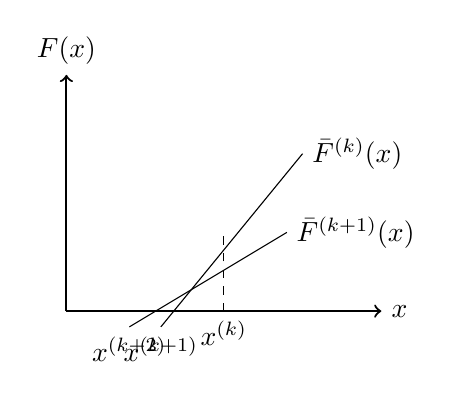
\begin{tikzpicture}
	\draw[thick,->] (0,0) -- (4,0) node[right]{$x$};
	\draw[thick,->] (0,0) -- (0,3) node[above]{$F(x)$};
	
	\draw (0.8, -0.2) node [below] {$x^{(k+2)}$} -- (2.8, 1) node [right] {$\bar{F}^{(k+1)}(x)$};
	\draw (1.2, -0.2) node [below] {$x^{(k+1)}$} -- (3, 2) node [right] {$\bar{F}^{(k)}(x)$};
	
	\draw [dashed] (2, 0) node [below] {$x^{(k)}$} -- ++(0,1);	
\end{tikzpicture} 

	\caption{Newton-Iteration}
\end{figure}

\subsubsection{Newton-Raphson-Verfahren} Die Idee hinter dem Newton-Raphson-Verfahren ist eine Taylorreihe erster Ordnung:
\[F(x) = F(x^{(k)}) + F'(x^{(k)}) \cdot (x - x^{(k)}) + F''(x^{(k)}) \cdot \frac{(x - x^{(k)})^2}{2} + \dots\]
\[x^{(k + 1)} = x^{(k)} - \frac{F(x^{(k)})}{F'(x^{(k)})}\]

Das Konvergenzverhalten des Newton-Raphson-Verfahrens erhält man aus einer Taylorreihe:
\[x^{(k + 1)} = x^{(k)} - \frac{F(x^\star) + F'(x^\star)(x^{(k)} - x^\star) + \frac{1}{2} F''(x^\star) \cdot {\epsilon^{k}}^2 + ... + \frac{1}{n!} F^{(n)}(x^\star) \cdot {\epsilon^{k}}^n}{F'(x^\star) + F''(x^\star) \cdot \epsilon^{(k)} + \frac{1}{(n - 1)!} \cdot F^{(n)} {\epsilon^{(k)}}^{n - 1}}\]
\[\epsilon^{(k + 1)} = \epsilon^{(k)} \left( 1 - \frac{F' + \frac{1}{2} F'' \cdot \epsilon^{(k)} + \dots}{F' + F'' \cdot \epsilon^{(k)} + \dots} \right) \approx \epsilon^{(k)} \left( \left(1 + \frac{1}{2} \epsilon^{(k)} \frac{F''}{F'} \right) \cdot \left( 1 - \frac{1}{2} \epsilon^{(k)} \frac{F''}{F'} \right) \right)\]
\[\epsilon^{(k + 1)} \approx \epsilon^{(k)} \left( 1 - \left( 1 + \frac{1}{2} \cdot \epsilon^{(k)} \frac{F''}{F'} - \epsilon^{(k)} \frac{F''}{F'}\right)\right) = \frac{1}{2} \cdot {\epsilon^{(k)}}^2 \frac{F''}{F'}\]

Probleme beim Newton-Raphson-Verfahren treten bei n-fachen Nullstellen ($F'(x^\star) = \dots = F^{(n - 1)}(x^\star) = 0)$, $F^{(n)}(x^\star) \ne 0$) auf.
\[\epsilon^{(k + 1)} \approx \epsilon^{(k)} \cdot \left( 1 - \frac{(n - 1)!}{n!}\right) - \epsilon^{(k)} \cdot \left( 1 - \frac{1}{n}\right) = \epsilon^{(k)} \frac{n - 1}{n}\]
Somit erhält man nur mehr lineare Konvergenz.
z.B.: $F(x) = e^x - 1 \Rightarrow x^{(k + 1)} = x^{(k)} - \frac{e^{x^{(k)}} - 1}{e^{x^{(k)}}}$

\paragraph{Variation: Sekanten-Methode}
\[F'(x^{(k)}) = \lim_{x \rightarrow x^{(k)}} \frac{F(x) - F(x^{(k)})}{x - x^{(k)}}\]
\[F'(x^{(k)}) = \frac{F(x^{(k - 1)}) - F(x^{(k)})}{x^{(k - 1)} - x^{(k)}}\]
Eingesetzt in die Newton-Gleichung erhält man somit
\[x^{(k + 1)} = x^{(k)} - \frac{F(x^{(k)}) \cdot (x^{(k)} - x^{(k - 1)})}{F(x^{(k)}) - F(x^{(k - 1)})}\]
Dadurch ist pro Schritt nur eine Funktionsauswertung nötig.


\subsection{Fixpunktiteration}
Fixpunkt $x^*$ einer Funktion $g(x)\cdot x^* = g(x^*)$.\\
Nullstellenproblem und Fixpunktproblem können ineinander überführt werden., z.B.
\[g(x) = x - F(x)\]

\subsubsection{Fixpunkttheorem}
\begin{enumerate}
	\item Sei $g(x)$ stetig auf $[a,b]$, sowie $g(x)\in [a,b]$ für alle $x\in [a,b]$.\\
	Dann hat $g(x)$ mindestens einen Fixpunkt auf $[a,b]$
	\item Existiere zusaätzlich $g'(x) auf (a,b)$, sowie eine positive Konstante $k<1$ mit $\abs{g'(x)}\leq k$, für alle $x\in (a,b)$
	\begin{itemize}
		\item Dann hat $g(x)$ exakt einen Fixpunkt auf $[a,b]$
		\item Gilt $0<k<1$, dann konvergiert für jedes $x^{(0)}\in [a,b]$ die Folge 
		\[x^{(n)} = g(x^{(n-1)})\quad,n\geq 1\]
		zum eindeutigen Fixpunkt $x^*\in [0,b]$.
	\end{itemize}
\end{enumerate}

\subsubsection{Konvergenzverhalten iterativer Verfahren}
\begin{align*}
	x^{(k+1)} &= g(x^{(k)}) & \text{Iterationsvorschrift}\\
	x^* &= g(x^*) & \text{Fixpunkt}
\end{align*}

Taylorreihe von $g(x)$ um $x^*$ 
\begin{align*}
	\left[g(x^{(k)})\right]x^{(k+1)} &= \underbrace{g(x^*)}_{x^*} + g'(x^*)\cdot (x^{(k)}-x^*) + \frac{1}{2} g''(x^*)\cdot (x^{(k)}-x^*)^2 + \ldots\\
	\varepsilon^{(k+1)} &= g'(x^*)\cdot \varepsilon^{(k)} + \frac{1}{2} g''(x^*)\cdot {\varepsilon^{(k)}}^2 + \ldots
\end{align*}
\begin{itemize}
	\item $g'(x^*)\neq 0$, $\abs{g'(x^*)} < 1 \quad\rightarrow$ lineare Konvergenz
	\item $g'(x^*) = 0$, $g''(x^*)\neq 0 \quad\Rightarrow$ quadratische Konvergenz ("Konstruktionshinweis")
\end{itemize}

\begin{figure}[htdp]
	\center
	\begin{tikzpicture}
	\draw[thick,->] (0,0) -- (4,0) node[right]{$x^{(i)}$};
	\draw[thick,->] (0,0) -- (0,4) node[above]{$x^{(i + 1)} = g(x^{(i)})$};
	
	\draw (0, -0) node [below] {$x^{(k+2)}$} -- (4, 4);
	\draw[blue,domain=0:4,name path=exp] plot (\x,{exp(0.3*\x)});
	
	\def\xZero{3.5}
	\def\xOne{2.85765111806316378986}
	\def\xTwo{2.35677777239982118523}
	\def\xThree{2.02796602315439250323}
	\def\xFour{1.83747033351067410687}
			
	\draw [dashed] (\xZero, 0) node [below] {$x^{(0)}$} -- (\xZero, \xOne);
	\draw [dashed] (0, \xOne) node [left] {$g(x^{(0)})$} -- (\xZero, \xOne);
	
	\draw [dashed] (\xOne, 0) node [below] {$x^{(1)}$} -- (\xOne, \xTwo);
	\draw [dashed] (0, \xTwo) node [left] {$g(x^{(1)})$} -- (\xOne, \xTwo);
	
	\draw [dashed] (\xTwo, 0) node [below] {$x^{(2)}$} -- (\xTwo, \xThree);
	\draw [dashed] (0, \xThree) node [left] {$g(x^{(2)})$} -- (\xTwo, \xThree);
	
	\draw [dashed] (\xThree, 0) node [below] {$x^{(3)}$} -- (\xThree, \xFour);
	\draw [dashed] (0, \xFour) node [left] {$g(x^{(3)})$} -- (\xThree, \xFour);
\end{tikzpicture} 

	\caption{Fixpunktiteration}
\end{figure}

\subsubsection{Mehrdimensionaler Newton}
\begin{align*}
	\vec{F}(\vec{x}) &= \vec{0}\quad,\vec{F} = (F_1,\ldots,F_r)^T\\
	\vec{F}(\vec{x}^{(k+1)}) &= \vec{F}(\vec{x}^{(k)}) + \underbrace{\frac{\partial\vec{F}(\vec{x}^{(k)})}{\partial\vec{x}^T}} \cdot\left(\vec{x}^{(k+1)}-\vec{x}^{(k)}\right)\\
	\begin{matrix}
	\text{Jacobi-Matrix}\\ \text{Fundamentalmatrix}
	\end{matrix}\qquad & \ma{J}(\vec{x}) = \frac{\partial\vec{F}(\vec{x})}{\partial\vec{x}^T} = \left(\frac{\partial\vec{F}}{\partial\vec{x}_1},\ldots,\frac{\partial\vec{F}}{\partial\vec{x}_r}\right) =\begin{pmatrix}
	\frac{\partial\vec{F}_1}{\partial\vec{x}_1} & \ldots & \frac{\partial\vec{F}_1}{\partial\vec{x}_r}\\
	\vdots & & \vdots\\
	\frac{\partial\vec{F}_r}{\partial\vec{x}_1} & \ldots & \frac{\partial\vec{F}_r}{\partial\vec{x}_r}
	\end{pmatrix}\\
	\vec{F}(\vec{x}^{(k+1)}) &= \vec{0}\Rightarrow\ma{J}(\vec{x}^{(k)})\cdot\left(\vec{x}^{(k+1)}-\vec{x}^{(k)}\right) = -\vec{F}(\vec{x}^{(1)})
\end{align*}
\[\vec{x}^{(k+1)} = \vec{x}^{(k)}-\ma{J}^{-1}(\vec{x}^{(k)})\cdot\vec{F}(\vec{x}^{(k)})\]
\textbf{Praktisch:}
\[\ma{J}(\vec{x}^{(k)})\cdot\vec{x}^{(k+1)} = \ma{J}(\vec{x}^{(k)})\cdot\vec{x}^{(k)} - \vec{F}(\vec{x}^{(k)})\]

\subsubsection{Konvergenz}
\[\vec x^{(k + 1)} = \vec \Phi(\vec x^{(k)}) = \vec \Phi(\vec x^\star) + \frac{\partial \vec \Phi}{\partial \vec x^T} \bigg|_{\vec x  = \vec x^\star} \cdot \left( \vec x^{(k)} - \vec x^\star \right) + \mathcal O\left( \left( \vec x^{(k)} - \vec x^\star \right) \cdot \left( \vec x^{(k)} - \vec x^\star \right)^T\right)\]

\[\vec \epsilon^{(k + 1)} = \frac{\partial \vec \Phi}{\partial \vec x^T} \bigg|_{\vec x = \vec x^\star} \vec \epsilon^{(k)} + \mathcal O \left( \vec \epsilon^{(k)} \cdot {\vec \epsilon^{(k)}}^T \right)\]

\[\vec \Phi(\vec x) = \vec x - \ma{J}^{-1} \cdot \vec F\]
\[\frac{\partial \vec \Phi}{\partial \vec x^T} = \underbrace{\ma{E} - \underbrace{\ma{J}^{-1} \underbrace{\frac{\partial \vec F}{\partial \vec x^T}}_{\ma J^{-1}}}_{\ma E}}_{\ma 0} - \underbrace{\frac{\partial \ma{J}^{-1}}{\partial \vec x^T} \cdot \vec F}_{\ma 0}\]

\subsubsection{Abbruchkriterien}
Gegeben sei eine Nullstellen-Suche: $\vec F(\vec x) = \vec 0 \Rightarrow \vec x^\star$

Als Abbruchkriterium wäre schön
\[||\vec x^{(k)} - \vec x^\star|| = || \vec \epsilon^{(k)} || \le || \vec \epsilon^{(A)} ||\]
oder
\[\frac{|| \vec \epsilon^{(k)} ||}{|| \vec x^\star ||} \le || \vec \epsilon^{(R)} ||\]
Problematisch dabei ist, dass $\vec x^\star$ unbekannt ist. Daher muss man in der Anwendung ein anderes Kriterium wählen:
\begin{itemize}
	\item $||\vec x^{(k + 1)} - \vec x^{(k)}|| \vec \epsilon^{(A)} ||$ bzw. $\frac{||\vec x^{(k + 1)} - \vec x^{(k)}||}{|| \vec x^{(k + 1)} ||} \le || \vec \epsilon^{(R)} ||$
	\item $||\vec F(\vec x^{(k + 1)}) - \vec F(\vec x^{(k)})|| \le \Delta_F^{(A)}$
	\item $||\vec F(\vec x^{(k)})|| \le F_{min}$
	\item $k > k_{max}$
\end{itemize}

\subsection{Allgemeines Iterationsverfahren für lineare Gleichungssysteme}
\begin{align*}
	\ma{A} \cdot \vec{x} &= \vec{b}\\
	\vec{x}^{(k+1)} &= \vec{\Phi} \left( \vec{x}^{(k)}\right)\\
	\ma{B} &\text{ beliebig}\\
	\ma{B} \cdot \vec{x} + \left( \ma{A} \cdot \ma{B} \right) \cdot \vec{x} &= \vec{b} \quad \\
	\Rightarrow \text{ Iterationsvorschrift:}&\\
	\ma{B} \cdot \vec{x}^{(k+1)} + \left(  \ma{A} - \ma{B} \right) \cdot \vec{x}^{(k)} &= \vec{b}\\
	\vec{x}^{(k+1)} &= \vec{x}^{(k)} - \ma{B}^{-1} \cdot \left( \ma{A} \cdot \vec{x}^{(k) - \vec{b}} \right) \\
	&= \underbrace{\left( \ma{I} - \ma{B}^{-1} \cdot \ma{A}\right)}_{\text{Konvergenz, wenn }|\lambda| < 1} \cdot \vec{x}^{(k)} + \ma{B}^{-1} \cdot \vec{b}
\end{align*}

\subsection{Iterative Verfahren zum Lösen linearer Gleichungssysteme}
\[\ma{A} \cdot \vec{x} = \vec{b},\ \ma{A} \in \mathrm{R}^{n\times n},\ \vec{x},\vec{b} \in \mathrm{R}^n,\ \ma{A} \text{ nicht singulär}\]

\begin{align*}
	\textbf{Splitting: } \ma{A} &= \begin{bmatrix}a_{ij}\end{bmatrix} = \ma{D} + \ma{L} + \ma{U}\\
	&= \begin{bmatrix}a_{11} & & & \\ & a_{22} & &\\ & & \ddots & \\ & & & a_{nn}\end{bmatrix} + 
	\begin{bmatrix}0 & & & \\ a_{21} & 0 & &\\ \vdots & & \ddots &  \\ a_{n1} & \ldots & a_{n\, n-1} & 0\end{bmatrix} + 
	\begin{bmatrix}0 & a_{12} & \ldots & a_{1n} \\ & 0 & & \vdots \\ & & \ddots & a_{n-1\,n} \\ & & & 0\end{bmatrix}
\end{align*}

\todo{Fix this !}

\begin{align*}
	\ma{A} &= \ma{S} - \ma{T}\\
	\ma{A} \cdot \vec{x} &= \left( \ma{S} - \ma{T} \right) \cdot \vec{x} = \vec{b}\\
	\Rightarrow \ma{S} \cdot \vec{x} &= \ma{T} \cdot \vec{x} + \vec{b}\\
	&= \left( \ma{S} - \ma{A} \right) \cdot \vec{x} + \vec{b}\\
	\Rightarrow \vec{x} &= \ma{S}^{-1} \cdot \left( \ma{S} - \ma{A} \right) \cdot \vec{x} + \ma{S}^{-1} \cdot \vec{b}
\end{align*}

\ldots

\subsubsection{Verschiedene Iterationsverfahren}
\begin{enumerate}
	\item $\ma{S} = \ma{D}\quad$ : Jacobi (Gesamtschrittverfahren)
	\item $\ma{S} = \ma{D}+\ma{L}\quad$ : Gauß-Seidl (Einzelschrittverfahren)
	\item $\ma{S} = \frac{1}{w}(\ma{D}+w\ma{L})\quad$ : sukzessive Überrelaxation (SOR, successive Over-Relaxation)
\end{enumerate}
\begin{enumerate}
	\item Jacobi: $\ma{S} = \ma{D};\ma{D}$ nicht singulär (d.h. $a_{ii}\neq 0$)
	\begin{align*}
		{A}\vec{x} = \vec{b}\Rightarrow\ma{D}\cdot\vec{x}^{(k+1)} &= (\ma{D}-\ma{A})\cdot\vec{x}^{(k)}+\vec{b} = (-\ma{L}-\ma{U})\cdot\vec{x}^{(k)}+\vec{b}\\
		\vec{x}^{(k+1)} &= \underbrace{\ma{D}^{-1}\cdot(-\ma{L}-\ma{U})}_{\ma{K}_j}\cdot\vec{x}^{(k)}+\underbrace{\ma{D}^{-1}\vec{b}}_{\vec{c}_j}\\
		&= \ma{K}_j\cdot\vec{x}^{(k)}+\vec{c}_j
	\end{align*}
	\item Gauss-Seidel: $\ma{S} = \ma{D} + \ma{L}$ (nicht singulär)
	\[\ma{A} \vec{x} + \vec{b} = \vec{0} \Rightarrow (\ma{D} + \ma{L}) \vec{x}^{(k + 1)} = (\ma{D} + \ma{L} - \ma{A}) \vec{x}^{(k)} + \vec{b} = -\ma{U} \vec{x}^{(k)} + \vec{b}\]
	\[\vec{x}^{(k + 1)} = \underbrace{-(\ma{D} + \ma{L})^{-1} \cdot \ma{U}}_{\ma{K}_g} \vec{x}^{(k)} + \underbrace{(\ma{D} + \ma{L})^{-1} \vec{b}}_{\vec{c}_g}\]
	\[\vec{x}^{(k + 1)} = \ma{K}_g \vec{x}^{(k)} + \vec{c}_g\]
	\item Successive Over-Relaxation: $\ma{S} = \frac{1}{\omega} (\ma{D} + \omega \ma{L})$
	\[\ma{A} \vec{x} = \vec{b}\]
	\[\frac{1}{\omega} (\ma{D} + \omega \ma{L}) \vec{x}^{(k + 1)} = \frac{1}{\omega} (\ma{D} + \omega \ma{L} - \ma{A}) \vec{x}^{(k)} + \vec{b}\]
	\[\ma{D} + \omega \ma{L}) \vec{x}^{(k + 1)} = (\ma{D} + \omega \ma{L} - \omega \ma{A}) \vec{x}^{(k)} + \omega \vec{b}\]
	\[\ma{D} + \omega \ma{L}) \vec{x}^{(k + 1)} = (\ma{D}(1 - \omega) - \omega \ma{U}) \vec{x}^{(k)} + \omega \vec{b}\]
	\[\vec{x}^{(k + 1)} = \underbrace{(\ma{D} + \omega \ma{L})^{-1} (\ma{D} (1 - \omega) - \omega \ma{U})}_{\ma{K}_\omega} \vec{x}^{(k)} + \underbrace{(\ma{D} + \omega \ma{L}) \omega \vec{b}}_{\vec{c}_\omega}\]
	\[\vec{x}^{(k + 1)} = \ma{K}_\omega \vec{x}^{(k)} + \vec{c}_\omega\]
	Die jeweilige Wahl von $\omega$ bei SOR beeinflusst dann das Konvergenzverhalten. Für Spezialfälle können Empfehlungen gegeben werden:
	\begin{enumerate}
		\item Falls $a_{ii} \ne 0$, $i = 1, \dots, n$ $\Rightarrow \varrho(\ma{K}_\omega) \ge |1 - \omega| \Rightarrow$ Konvergenz für $0 < \omega < 2$
		\item Falls $\ma{A}$ positiv definit und $0 < \omega < 2$, dann konvergiert SOR für jede Initiallösung $\vec{x}^{(0)}$
		\item Falls $\ma{A}$ positiv definit und tridiagonal ist, dann $\varrho(\ma{K}_g) = \varrho(\ma{K}_j)^2 < 1$ und die optimale Wahl für $\omega$ ist:
		\[\omega = \frac{2}{1 + \sqrt{1 - \varrho(\ma{K}_j)^2}}\]
	\end{enumerate}
\end{enumerate}
Ein Beispiel zum Vergleich zwischen Jacobi und Gauß-Seidel
\begin{align*}
	10 &x_1 - &x_2 + 2 &x_3 & &= 6 \\
	- &x_1 + 11 &x_2 - &x_3 + 3 &x_4 &= 25 \\
	2 &x_1 - &x_2 + 10 &x_3 - &x_4 &= -11 \\
	& 3 &x_2 - &x_3 + 8 &x_4 &= 15
\end{align*}

Jacobi:
\begin{align*}
	x_1^{(k + 1)} &= \frac{1}{10} x_2^{(k)} - \frac{1}{5} x_3^{(k)} + \frac{3}{5} \\
	x_2^{(k + 1)} &= \frac{1}{10} x_1^{(k)} + \frac{1}{11} x_3^{(k)} - \frac{3}{11} x_4^{(k)} + \frac{25}{11} \\
	x_3^{(k + 1)} &=  -\frac{1}{5} x_1^{(k)} + \frac{1}{10} x_2^{(k)} + \frac{1}{10} x_4^{(k)} - \frac{11}{10} \\
	x_4^{(k + 1)} &= \frac{3}{8} x_2^{(k)} + \frac{1}{8} x_3^{(k)} + \frac{15}{8}
\end{align*}

Gauß-Seidel:
\begin{align*}
	x_1^{(k + 1)} &= & \frac{1}{10} x_2^{(k)} - \frac{1}{5} x_3^{(k)} + \frac{3}{5} \\
	x_2^{(k + 1)} &= \frac{1}{11} x_1^{(k + 1)} + & \frac{1}{11} x_3^{(k)} - \frac{3}{11} x_4^{(k)} + \frac{25}{11} \\
	x_3^{(k + 1)} &= -\frac{1}{5} x_1^{(k + 1)} + & \frac{1}{10} x_2^{(k + 1)} + \frac{1}{10} x_4^{(k)} - \frac{11}{10} \\
	x_4^{(k + 1)} &= & \frac{3}{8} x_2^{(k + 1)} + \frac{1}{8} x_3^{(k + 1)} + \frac{15}{8}
\end{align*}
Man erkennt bei Gauß-Seidel die Abhängigkeit von Werten, welche erst im aktuellen Iterationsschritt berechnet werden. In der Praxis bietet Gauß-Seidel dadurch in der Regel eine schneller Konvergenz. Vorteil von Jacobi ist jedoch die bessere Parallelisierbarkeit eines Iterationsschrittes.

\paragraph{Konvergenzbetrachtung}
\begin{equation}
	\ma{S} \vec{x} = \ma{T} \vec{x} + \vec{b}
	\label{eq:jacobi_konvergenz_1}
\end{equation}
\begin{equation}
	\ma{S} \vec{x}^{(x + 1)} = \ma{T} \vec{x}^{(k)} + \vec{b}
	\label{eq:jacobi_konvergenz_2}
\end{equation}

\ref{eq:jacobi_konvergenz_1} - \ref{eq:jacobi_konvergenz_2}:
\[\ma{S} (\vec{x} - \vec{x}^{(k + 1)}) = \vec{T} (\vec{x} - \vec{x}^{(k)})\]
\[\ma{S} \vec{e}^{(k + 1)} = \ma{T} \vec{e}^{(k)}\]
\[\vec{e}^{(k + 1)} = \ma{S}^{-1} \ma{T} \vec{e}^{(k)}\]
\[\vec{e}^{(k + 1)} = \ma{G} \vec{e}^{(k)} = \ma{G}^k \vec{e}^{(0)}\]

\subsection{Gradientenverfahren}
Sei $ \ma{A} \in \mathbb{R}^{n\times n} $ mit
\begin{itemize}
	\item $\ma{A}^T = \ma{A}$
	\item $\vec{x}^T \cdot \ma{A} \cdot \vec{x} > 0$ für $\vec{x} \neq 0$ (positiv definit)
	\item $\vec{b} \in \mathbb{R}$
\end{itemize}

Dann existiert genau ein Minimum für die quadratische Form:
\begin{align*}
	\Phi(\vec{x}) &= \num{0.5} \cdot \vec{x}^T \cdot \ma{A} \cdot \vec{x} - \vec{x}^T \cdot \vec{b}\\
	\nabla \Phi(\vec{x}) &= \num{0.5} \left( \ma{A}^T + \ma{A} \right) \cdot \vec{x} - \vec{b} = \ma{A} \cdot \vec{x} - \vec{b}\\
	\text{Minimum: } \nabla \Phi(\vec{x}) = \vec{0} \Rightarrow \ma{A} \cdot \vec{x} = \vec{b}
\end{align*}

$\Rightarrow$ Minimierung der quadratischen Form entspricht Lösung des linearen Gleichungssystem.

\subsection{Iterativer Ansatz für Minimierungsproblem}
\begin{tabular}{ll}
	\textbf{Allgemein:} & $\vec{x}^{(k+1)} = \vec{x}^{(k)} + \alpha_K \cdot \vec{d}^{(k)}$\\
	\textbf{Bestimme:} & $\alpha_k,\ \vec{d} = ?$\\
	\textbf{Idee:} & Wähle Richtung des steilsten Abstiegs ("'sleepest descent"', siehe \autoref{fig:sleepest-descent})\\
\end{tabular}

\begin{figure}[htdp]
	\center
	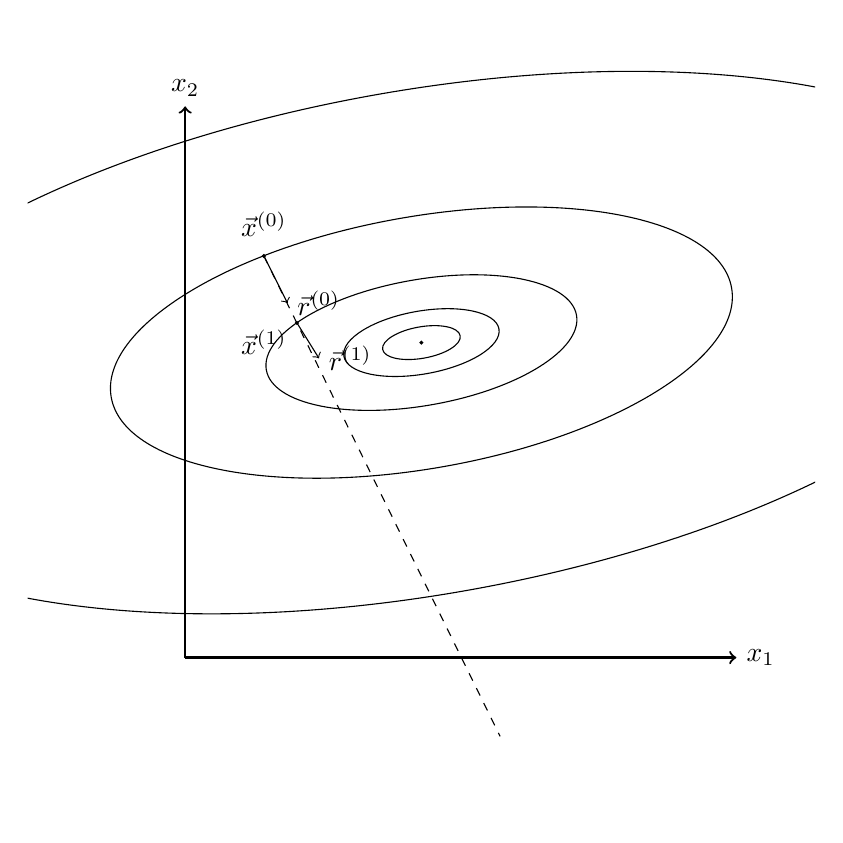
\begin{tikzpicture}	
	\coordinate (center) at (3, 4);
	
	\clip (-2, -2) -- (8, -2) -- (8, 8) -- (-2, 8) -- (-2, -2);
	\draw[thick,->] (0,0) -- (7,0) node[right]{$x_1$};
	\draw[thick,->] (0,0) -- (0,7) node[above]{$x_2$};
	\node[draw,circle,inner sep=0.2pt,fill,black] at (center) {};
	\draw[rotate=10] (center) ellipse (0.5cm and 0.2cm);
	\draw[rotate=10] (center) ellipse (1cm and 0.4cm);
	\draw[rotate=10] (center) ellipse (2cm and 0.8cm);
	\draw[rotate=10] (center) ellipse (4cm and 1.6cm);
	\draw[rotate=10] (center) ellipse (8cm and 3.2cm);
	
	\node[draw,circle,inner sep=0.2pt,fill,black] at (1, 5.1) {};
	\node at (1, 5.5) {$\vec{x}^{(0)}$};
	\draw[->] (1, 5.1) -- (1.3, 4.5) node[right] {$\vec{r}^{(0)}$};
	\draw[thin, dashed] (1, 5.1) -- (4, -1) node[right] {};
	\node[draw,circle,inner sep=0.2pt,fill,black] at (1.42, 4.25) {};
	\node at (1, 4) {$\vec{x}^{(1)}$};
	\draw[->] (1.42, 4.25) -- (1.7, 3.8) node[right] {$\vec{r}^{(1)}$};

\end{tikzpicture} 

	\caption{Gradientenverfahren - sleepest descent}
	\label{fig:sleepest-descent}
\end{figure}

\begin{align*}
	\vec{d}^{(k)} &= - \nabla \Phi(\vec{x}^{(k)}) = \vec{b} \cdot \ma{A} \cdot \vec{x}^{(k)} =: \vec{r}^{(k)} \text{ Residium}\\
\end{align*}
$\alpha_k = ? \quad \Rightarrow $ Minimiere $ \vec{\Phi}$\\
\begin{align*}
	\vec{x}^{(k+1)} &= \vec{x}^{(k)} + \alpha_k \vec{r}^{(k)}\\
	\vec{\Phi}(x^{(k+1)}) &= \frac{1}{2} \left( \vec{x}^{(k)} + \alpha_k \vec{r}^{(k)}\right)^T \cdot \ma{A} \cdot \left( \vec{x}^{(k)} + \alpha_k \vec{r}^{(k)}\right) - \left( \vec{x}^{(k)} + \alpha_k \vec{r}^{(k)}\right)^T \cdot \vec{b}\\
	\frac{\partial \vec{\Phi}(x^{(k+1)})}{\partial \alpha_k} &= \frac{1}{2} {\vec{r}^{(k)}}^T \cdot \ma{A} \cdot \vec{x}^{(k)} + \frac{1}{2} {\vec{x}^{(k)}}^T \cdot \ma{A} \cdot \vec{r}^{(k)} + \alpha_k \cdot {\vec{r}^{(k)}}^T \cdot \ma{A} \cdot \vec{r}^{(k)} - {\vec{r}^{(k)}}^T \cdot \vec{b}\\
	&= {\vec{r}^{(k)}}^T \cdot \ma{A} \vec{x}^{(k)} - {\vec{r}^{(k)}}^T \cdot \vec{b} + \alpha_k \cdot {\vec{r}^{(k)}}^T \cdot \ma{A} \cdot \vec{r}^{(k)} \neq 0\\
	\ldots\\
	\Rightarrow \alpha &= \frac{{\vec{r}^{(k)}}^T \cdot \vec{r}^{(k)}}{{\vec{r}^{(k)}}^T \cdot \ma{A} \cdot \vec{r}^{(k)}}\\
	\textbf{Verfahren: } k &= 0,1,2,\ldots\\
	\vec{r}^{(k)} &= \vec{b} \cdot \ma{A} \cdot \vec{x}^{(k)}\\
	\alpha_k &= \frac{{\vec{r}^{(k)}}^T \cdot \vec{r}^{(k)}}{{\vec{r}^{(k)}}^T \cdot \ma{A} \cdot \vec{r}^{(k)}}\\
	\vec{x}^{(k+1)} &= \vec{x}^{(k)} + \alpha_k \cdot \vec{r}^{(k)}
\end{align*}

2 Matrix-Vektormultiplikationen (dominant)\\
2 Vektor-Skalarprodukte\\
Alternative:\\
\begin{align*}
	- \ma{A} \cdot \vec{x}^{(k+1)} + \vec{b} &= - \ma{A} \cdot \vec{x}^{(k)} - \alpha_k \cdot \ma{A} \cdot \vec{r}^{(k)} + \vec{b}\\
	\vec{r}^{(k+1)} &= \vec{r}^{(k)} - \alpha_k \cdot \ma{A} \vec{r}^{(k)}\\
	\Rightarrow \text{ nur eine Matrix-Vektormultiplikation je Iteration}
\end{align*}

\subsection{Konvergenz}
\begin{align*}
	\vec{x}^{(k)} &= \vec{x}^* + \vec{e}^{(k)} \text{, Annahme: } \vec{e} \text{ is EV von } \ma{A}:\\
	\ma{A} \cdot \vec{e} &= \lambda_e \cdot \vec{e}\\
	\vec{r}^{(k)} &= \vec{b} - \ma{A} \cdot \vec{x}^{(k)}\\
	&= \vec{b} - \ma{A} \cdot \left( \vec{x}^* + \vec{e}^{(k)}\right)\\
	&= \underbrace{\vec{b} - \ma{A} \cdot \vec{x}^*}_{\vec{0}} - \ma{A} \cdot \vec{e}^{(k)}\\
	\vec{r}^{(k)} &= - \ma{A} \cdot \vec{e}^{(k)} = - \lambda_e \cdot \vec{e}^{(k)} \Rightarrow \vec{r}^{(k)} \text{ ist ebenfalls EV}
\end{align*}

\begin{align*}
\text{Aus (3): } \vec{x}^{(k+1)} &= \vec{x}^{(k)} + \alpha_k \cdot \vec{r}^{(k)}\\
\vec{e}^{(k+1)} &= \vec{e}^{(k)} + \alpha_k \cdot \vec{r}^{(k)}\\
&= \vec{e}^{(k)} + \frac{{\vec{r}^{(k)}}^T \cdot \vec{r}^{(k)}}{{\vec{r}^{(k)}}^T \cdot \ma{A} \cdot \vec{r}^{(k)}} \cdot \left( -\lambda_e \cdot \vec{e}^{(k)}\right)\\
&= \vec{e}^{(k)} + \frac{{\vec{r}^{(k)}}^T \cdot \vec{r}^{(k)}}{{\vec{r}^{(k)}}^T \cdot \vec{r}^{(k)} \cdot \lambda_e} \cdot \left( -\lambda_e \cdot \vec{e}^{(k)}\right)\\
&= \vec{e}^{(k)} - \vec{e}^{(k)} = \vec{0} \Rightarrow \text{Exakte Lösung in einem Schritt}
\end{align*}

\textbf{Allgemein}

\begin{align*}
||\vec{x}||_A &= \sqrt{\vec{x}^T \cdot \ma{A} \cdot \vec{x}} \text{ Energienorm}\\
\text{Es gilt: } ||\vec{e}^{(k+1)}||_A &= \frac{k_2(\ma{A})-1}{k_2(\ma{A})+1} \cdot ||\vec{e}^{(k)}||_A
\end{align*}

\subsection{CG - Konjugierte Gradientenmethode}
$ \vec{p}^{(k)} $ ist eine Menge mit $ \underbrace{{\vec{p}^{(i)}}^T}_{\text{paarweise A-orthogonal bzw. A-konjugiert}} \cdot \ma{A} \cdot \vec{p}^{(j)} = 0, \forall i,j=1,\ldots,n\quad i \neq j$\\
$ \Rightarrow \vec{p}^{(k)}$ bilden eine Basis des $\mathbb{R}^n$

\begin{align*}
\text{Daher: } \vec{x}^* &= \sum^n_{i=1} \alpha_i \cdot \vec{p}^{(i)}\\
\Rightarrow \vec{b} &= \ma{A} \cdot \vec{x}^* = \sum^n_{i=1} \alpha_i \cdot \ma{A} \cdot \vec{p}^{(i)}
\end{align*}

\subsubsection{Schrittweite}
\begin{align*}
0 = \frac{\partial\vec{\Phi}}{\partial\alpha_k}\left(\vec{x}^{(k)}+\alpha_k\vec{p}^{(k)}\right)\\
\Rightarrow\alpha_k = \frac{{\vec{p}^{(k)}}^T\cdot\vec{r}^{(k)}}{{\vec{p}^{(k)}}^T\cdot\ma{A}\cdot\vec{p}^{(k)}}
\end{align*}
Wie Gradientenverfahren, aber Suchrichtung $\vec{p}$

\subsubsection{Suchrichtung}
\textbf{Definition:} Lösung $\vec{x}^{(k)}$ heißt optimal bzgl. einer Richtung $\vec{p}\neq 0$, wenn $\vec{\Phi}(\vec{x}^{(k)})\leq\vec{\Phi}(\vec{x}^{(k)}+\lambda\vec{p})\;,\;\forall\lambda\in\R$\\
\begin{itemize}
\item[$\Leftrightarrow$] $\vec{\Phi}$ besitzt lokales Minimum entlang $\vec{p}$ für $\lambda = 0$
\item[$\Leftrightarrow$] $\frac{\partial\vec{\Phi}}{\partial\lambda}\left(\vec{x}^{(k)}+\lambda\vec{p}^{(k)}\right)\vert_{\lambda = 0} = \vec{p}^T\cdot\ma{A}\cdot\vec{x}^{(k)} - \vec{p}\vec{b}^T + \lambda\vec{p}^T\cdot\ma{A}\cdot\vec{p}\vert_{\lambda = 0}$
\item[$\Leftrightarrow$] $\vec{p}\vec{I}\vec{r}^{(k)}$
\end{itemize}
\begin{align*}
\text{Sei }\vec{x}^{(k+1)} = \vec{x}^{(k)} + \vec{q}\Rightarrow\vec{r}^{(k+1)} &= \vec{b}\cdot\ma{A}\cdot\vec{x}^{(k+1)}\\
&= \vec{b}\cdot\ma{A}\cdot\vec{x}^{(k)} - \ma{A}\vec{q}\\
&= \vec{r}^{(k)} - \ma{A}\vec{q}
\end{align*} 
Forderung $\vec{x}^{(k+1)}$ ebenfalls optimal bzgl. $\vec{p}$, also
\begin{align*}
0 = \vec{p}^T\cdot\vec{r}^{(k+1)} &= \vec{p}^T\cdot(\vec{r}^{(k)} - \ma{A}\vec{q})\\
&= \underbrace{\vec{p}^T\cdot\vec{r}^{(k)}}_{0}-\vec{p}^T\cdot\ma{A}\cdot\vec{q} = \underbrace{-\vec{p}^T\cdot\ma{A}\cdot\vec{q}}_{\vec{p},\vec{q},\ma{A}\text{orthogonal}} = 0
\end{align*}

\textbf{Konstruktion der Suchrichtung}
\begin{itemize}
\item Start $\vec{p}^{(0)} = \vec{r}^{(0)}$ (Ausgehend von Initiallösung $\vec{x}^{(0)}$, Gradient an $\vec{x}^{(0)}$)
\item Suche Richtungen $\vec{p}^{(k+1)} = \vec{r}^{(k+1)} - \beta_k\cdot\vec{p}^{(k)}\;,k=0,1,2,\ldots$ mit $\beta_k\in\R$, so dass gilt:
\begin{align*}
{\vec{p}^{(j)}}^T\cdot\ma{A}\cdot\vec{p}^{(k+1)} = 0 = {\left(\ma{A}\cdot\vec{p}^{(j)}\right)}^T\cdot\vec{p}^{(k+1)} = 0\;,j=0,1,\ldots,k\\
\Rightarrow {\left(\ma{A}\cdot\vec{p}^{(j)}\right)}^T\cdot\left(\vec{r}^{(k+1)}-\beta_k\cdot\vec{p}^{(k)}\right) = 0 \underset{(j=k)}{\Rightarrow}\beta_k = \frac{\left(\ma{A}\cdot\vec{p}^{(k)}\right)^T\cdot\vec{r}^{(k+1)}}{\left(\ma{A}\cdot\vec{p}^{(k)}\right)^T\cdot\vec{p}^{(k)}}
\end{align*}
\end{itemize}
Zu zeigen: $\vec{p}^{(k+1)}$ ist $\ma{A}$ orthogonal zu $\vec{p}^{(j)}\;\forall j<k$\\
Beweisidee: vollständige Induktion
